\subsubsection{Stufenindex}

Der Stufenindex ist durchsatzschwächste Brechzahlprofil (ca. 100 Megabit/s auf
100 m). In \autoref{subsec:poffunktionsweise} wurde die Funktionsweise von
optischen Wellenleitern an diesem Profil erklärt. Als Kernmaterial wird
Polymethylmethacrylat (PMMA, siehe \autoref{subsec:pofpmma}) eingesetzt
\cite{pofacsi}. \autoref{fig:pofsi} fasst den Aufbau und die Lichtausbreitung
zusammen. Die Spalte mit Brechungsindex als Überschrift stellt den Verlauf
dieses grafisch dar. Beim Stufenindexprofil steigen die Brechzahlen beim
Übergang vom Mantel zum Kern abrupt an. Dies hat die schon erwähnte
Totalreflexion an der Kerngrenze, welche man in der Spalte Querschnitt erkennen
kann, zur Folge.

\begin{figure}[h]
    \begin{center}
        \begin{minipage}[t]{0.4\textwidth}
            \begin{center}
                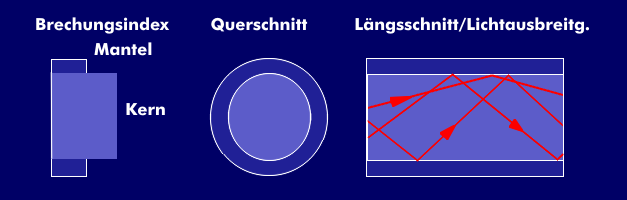
\includegraphics[height=0.1\textheight]{Bilder/Optische_Wellenleiter_Die_Polymer_Optische_Faser/Brechzahlprofile/pofsi.png}
                \caption[Aufbau des Stufenindexprofils \newline \url{ITWissen}]{Aufbau des Stufenindexprofils}
                \label{fig:pofsi}
            \end{center}
        \end{minipage}
    \end{center}
\end{figure}

%TODO: Modify picture, enhance reference for sections, get url
